%----------------------------------------------------------------------------------------
%	HEADER
%----------------------------------------------------------------------------------------
% !TeX spellcheck = en_US

\documentclass[12pt, a4paper, oneside]{article}

\usepackage[english]{babel} % Language hyphenation and typographical rules

\usepackage[top=3cm, left=3cm, right=2cm, bottom=2.5cm]{geometry} % Document margins
\usepackage[hang, small,labelfont=bf,up,textfont=it,up]{caption} % Custom captions under/above floats in tables or figures
\usepackage{booktabs} % Horizontal rules in tables

\usepackage{lettrine} % The lettrine is the first enlarged letter at the beginning of the text

\usepackage{enumitem} % Customized lists
\setlist[itemize]{noitemsep} % Make itemize lists more compact

% TODO do we need a abstract?
\usepackage{abstract} % Allows abstract customization
\renewcommand{\abstractnamefont}{\normalfont\bfseries} % Set the "Abstract" text to bold
\renewcommand{\abstracttextfont}{\normalfont\small\itshape} % Set the abstract itself to small italic text

\usepackage{titlesec} % Allows customization of titles
%\renewcommand\thesection{\Roman{section}} % Roman numerals for the sections
\titleformat{\section}[block]{\large\scshape\centering}{\thesection.}{1em}{} % Change the look of the section titles
\titleformat{\subsection}[block]{\large}{\thesubsection.}{1em}{} % Change the look of the section titles

\usepackage{fancyhdr} % Headers and footers
\pagestyle{fancy} % All pages have headers and footers
\fancyhead{} % Blank out the default header
\fancyfoot{} % Blank out the default footer
\fancyhead[C]{Water Management $\bullet$ Seminar Computational Economics $\bullet$ Winter Semester 2019/2020} % Custom header text
\fancyfoot[RO,LE]{\thepage} % Custom footer text

\setlength{\parindent}{0em}

\usepackage{titling} % Customizing the title section

\usepackage{hyperref} % For hyperlinks in the PDF

\usepackage{graphicx} % for figures

\usepackage{longtable}

% packages used for citations
\usepackage[
backend=bibtex,
style=alphabetic,
citestyle=authoryear,
natbib=true
]{biblatex}
\addbibresource{collection.bib}

% TODO delete the lorem ipsum
\usepackage{blindtext} % Package to generate dummy text throughout this template 

\title{Water Management}
%----------------------------------------------------------------------------------------

\begin{document}
	
	%----------------------------------------------------------------------------------------
	%	COVER SHEET
	%----------------------------------------------------------------------------------------
	
	\begin{titlepage}
		\begin{center}
			\vspace*{1cm}
			
			\textbf{Seminar \textit{Computational Economics}}                
			
			\vspace{0.5cm}
			{\makeatletter{\@title}\makeatother}
			
			\vspace{1.5cm}
			
			\textbf{Felix Fink} \\
			stud. 2nd semester M.Sc. Business Administration and Engineering: Mechanical Engineering \\
			Matr. Nr. 345971 \\
			\href{mailto:felix.fink@rwth-aachen.de}{felix.fink@rwth-aachen.de} 
			
			\vspace{1cm}
			
			\textbf{Niklas Sayer} \\
			stud. 2nd semester M.Sc. Business Administration and Engineering: Materials- and Process Engineering\\
			Matr. Nr. 332404
			\href{mailto:niklas.sayer@rwth-aachen.de}{niklas.sayer@rwth-aachen.de} 
			
			\vspace{1cm}
			
			\textbf{Martin Wicke} \\
			stud. M.Sc. Business Administration and Engineering: Electrical Power Engineering\\
			Matr. Nr. 336301 \\
			\href{mailto:martin.wicke@rwth-aachen.de}{martin.wicke@rwth-aachen.de} 
			
			\vfill
			
			
			Supervisor\\
			Thomas Gehrmann, M.Sc.
			
			\vspace{0.8cm}
			
			%\includegraphics[width=0.4\textwidth]{university}
			
			Computational Economics\\
			RWTH Aachen University\\
			Winter Semester 2019/2020
			
		\end{center}
	\end{titlepage}

	%----------------------------------------------------------------------------------------
	%	TABLE OF CONTENTS
	%----------------------------------------------------------------------------------------
	
	\tableofcontents
	\clearpage
	
	%----------------------------------------------------------------------------------------
	%	ARTICLE CONTENTS
	%----------------------------------------------------------------------------------------
	
	\section{Introduction}
	
	\subsection{Motivation}
With world population expected to hit 9.7 billion in 2050 and 11.2 billion in 2100, more and more people will have to be fed, which will increase the demand of water for agriculture uses \citep{un2019}.
Already today, around one third of the world's population live under physical water scarcity \citep{vorosmarty2000global, alcamo2003global, oki2006global}.
With climate change proceeding, rainfall as the natural influx of lakes will become more volatile in some regions while prolonged dry periods will make water an even more precious resource in other areas \citep{guhathakurta2011impact}.
This situation will get even worse due to the projected increase in the demand of water per capita in many regions of the world, driven by lifestyle factors, especially diet \citep{vorosmarty2000global}.
Despite all those challenges, research suggests that just by using water more efficiently, we will be able to meet the acute water, environment and poverty challenges facing us over the next 50 years \citep{molden2013water}.
Therefore, the optimal allocation and sustainable use of the available water will be of increasing importance in the future.


\subsection{Assumptions and Conditions}

In this work we want to examine the variations in use of water from a (hypothetical) water reservoir.
One of the most important uses of surface water is the irrigation of fields for food production. However, as farming and food production are private enterprises and lakes are public goods, interests of all different parties have to be considered.
The water reservoir to be considered has two stakeholders: farmers, who want to use the water for irrigation purposes and citizens, who want to use the lake for recreational activities.
Note that while looking at just two agents is a vast simplification compared to a real allocation problem, one can easily add more stakeholders to the model, as long as there is enough computational power.
The sequence of events for every period is displayed in figure ~\ref{fig:Sequence}.
At the beginning of every year (Step 1) we have to decide how much of the water from the reservoir is used for the irrigation of fields, which benefits the farmers' harvest.\\\\
The farmers utility function follows the form 

\begin{equation}
	F(x) = \frac{a_1}{1+b_1} * x^{1+b_1}
\end{equation}

where $x$ represents the amount of water to be used for irrigation in a year. The preference parameters are $a_1 = 1$ and $b_1 = -2$.\\\\

During the summer months, citizens benefit from the remaining water due to recreational use (Step 2).
This can be described by the recreational users' utility function which is

\begin{equation}
  G(s, x) = \frac{a_2}{1+b_2} * (s-x)^{1+b_2}
\end{equation}

with the additional paramter $s$ that indicates the water level at the beginning of the year.
For recreational users, the preference parameters shell be $a_2 = 2$ and $b_2 = -3$.\\\\

At the end of the year, water in the reservoir is replenished by rainfall (Step 3), which we can assume to be randomly following a lognormal distribution \citep{oosterbaan1994frequency}:
\begin{equation}
	r \sim lognormal(\mu, \sigma^2)
\end{equation}

with parameters $\mu = 0$ and $\sigma^2 = 1$.\\\\

Other parameters are the maximum capacity of the reservoir
\begin{equation}
	M = 7
\end{equation}

and the discount factor for future utility 

\begin{equation}
	\beta = 0.9
\end{equation}

\begin{figure}[ht]
	\includegraphics[width=1\textwidth]{figures/CESchaubild_Cut.png}
	\caption{Sequence of Events in One Period}
	\label{fig:Sequence}
\end{figure}

Using dynamic programming in combination with a stochastic simulation of the rainfall, we determined the optimal irrigation policy that maximizes the combined utility of farmers and citizens for a number of years $T$.
In the main part we will give a brief summary of the underlying theory and the optimization problem.
After that we will present the results and our conclusions for the original model and its modifications, as well as possible shortfalls of our analysis.
At the end we also give a little outlook into further possible extensions.


\subsubsection{Modification 1: Variation of the Discount Factor}
We also study the effects of different betas on the optimal irrigation policy. 
The discount factor takes into account that agents in a simple two-stage model often value current consumption over future consumption.
It expresses how much one unit of future utility is worth in terms of current utility and therefore makes them easily comparable \citep{kruschwitz2014investitionsrechnung}.
We take a look at the discount factors x and x.

\subsubsection{Modification 2: Increased Rainfall Volatility}
To consider the predicted impacts of climate change \citep{guhathakurta2011impact}, we look at the effect of increased rainfall volatility. 
We do this by using a  $\sigma^2$ of x.

\subsubsection{Modification 3: Using Real Data for Rainfall}
Instead of simulating the rainfall with random numbers, we also use real data.
Comparing the results then allows us to draw conclusions on the accuracy of the simulation for that region. 
We use a dataset aquired from \cite{kaggle:2019}, that contains real rainfall data for the four main water reservoirs of the city Chennai, India. % Zitation anpassen

\subsubsection{Modification 4: Taking Evaporation into Account}
The evaporation of water from a water reservoir is the most important natural "outflow" to be considered when it comes to managing water levels \citep{tanny2008evaporation}.
It therefore should definitely be considered in a real model that is used to determine the optimal irrigation strategy.
The dataset that we use for the real rainfall also contains the water levels of the four reservoirs.
Using these values together, we calculate the evaporation of water and include it in our model. \\\\


Note that all modifications, except Modification 4, are based on the original model without any modifications.
Modification 4 is an extension of Modification 3. 

	%------------------------------------------------
	
	\section{Main Part}
	\subsection{Theory}
	
	In this paper, the theoretical knowledge obtained in the seminar shall be applied. 
	
	\subsubsection{Quadrature}
	In many computational applications, formulas 	are used to calculate values of any kind. For example, let the flow of water through a pipe be 

	\begin{equation}
	f(t) = sin(\pi t), \; t \in [0,1]
	\end{equation}

Now, it's trivial to compute the flow at any given time using code, simply by implementing the formula as given above. However, if we want to compute the amount of water flowing through the pipe in the time interval $[0.25, 0.5]$, we can not calculate that directly, as we would have to know the antiderivative of $f(t)$. Apart from this example, it's not always trivial to calculate the antiderivative of a function analytically. However it is possible compute the area below (almost) any function using numerical integration, also called numerical quadrature. 

A naive implementation of a quadrature could be to calculate the total area of equidistant rectangles whose height corresponds to the function value of $f$: 

	\begin{figure}[ht] 
		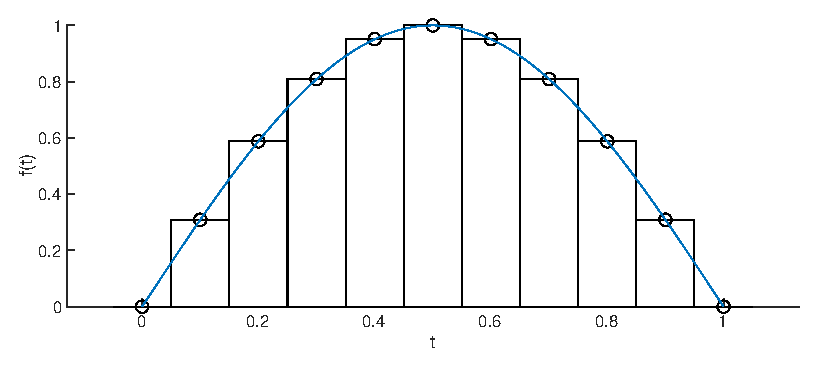
\includegraphics[width=1\textwidth]{figures/quadratureA.eps}
		\caption{Quadrature using Midpoint Rule}
		\label{fig:quadrature-a}
	\end{figure}
This implementation of a quadrature is called \emph{Midpoint Rule}. 
\\

A more sophisticated way to determine the area of an unbounded integral is to use the Gauss-Hermite Formula

	\begin{equation}
	\int_{-\infty}^{\infty} f(x)e^{-x^2} dx \approx \sum_{i=1}^{n}{w_if(x_i)}
	\end{equation}

where the weights $w_i$ are given as the solution to a linear system of equations and the nodes $x_i$ correspond to the zeros of the nth Hermite polynomial. \cite{seminar:week6}

	\subsection{bla}
	\begin{figure}[ht] % TODO remove example
		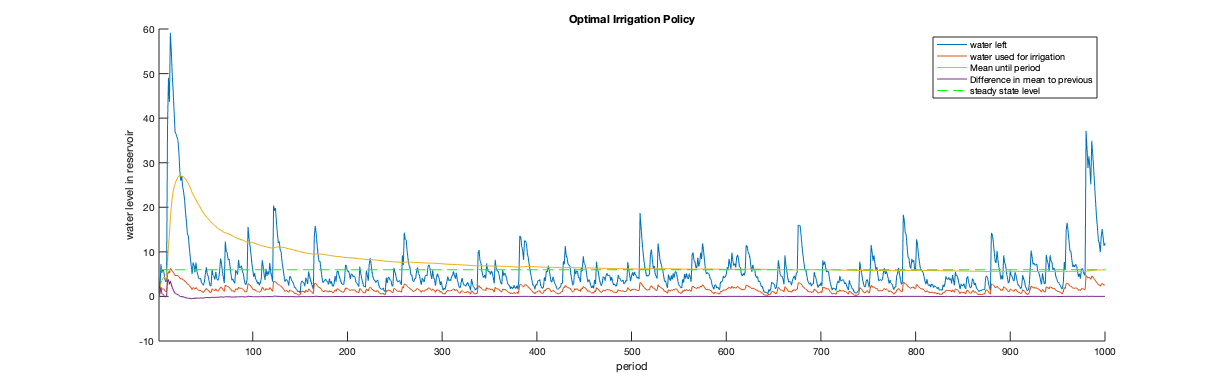
\includegraphics[width=1\textwidth]{figures/example.png}
		\caption{Example Image}
		\label{fig:example-pic}
	\end{figure}
	\blindtext
	\begin{figure}[ht] % TODO remove example
		\begin{longtable}{|p{2,5cm}|p{2,5cm}|p{2,5cm}|p{3cm}|p{3cm}|}
			\hline
			&\multicolumn{4}{c|}{\textbf{Klasse}} \\
			\hline
			& \textbf{S0} & \textbf{S1} & \textbf{S2} & \textbf{S3} \\
			\hline
			\textbf{lorem} & ipsum & ipsum & ipsum & ipsum \\
			\hline
		\end{longtable}
		\label{fig:example-figure}
		\caption{Example Table}
	\end{figure}
	\blindtext
	\blindtext
	\blindtext
	
	%------------------------------------------------
	
	\section{Conclusion}
	This chapter will discuss the outcomes and results of the implemented functionality in MATLAB.
	The discussion will be started on the basic questions asked by the project description.
	Furthermore we made several modifications to the task which will be discussed additionally.
	All results will be visualized by plots made within our simulation in MATLAB.
	\subsection{Optimal irrigation policy}
	When questioning what the optimal irrigation policy is, the first question to be asked is how the aggregated value function of both recreational users and farmers looks like.
	The value function as posed in % TODO put links to theory here
	contains the maximum possible usage that can be gained by irrigating a specific amount of water under a given water level. 
	\ref{fig:value-function} show the value function calculated for all possible water levels between the allowed boundaries of 0 and 7.
	The plot shows a rising proposed irrigation amount with rising water level up to a water level of approximately 1.5 where a declining irrigation amount is favored.
	\begin{figure}[ht]
		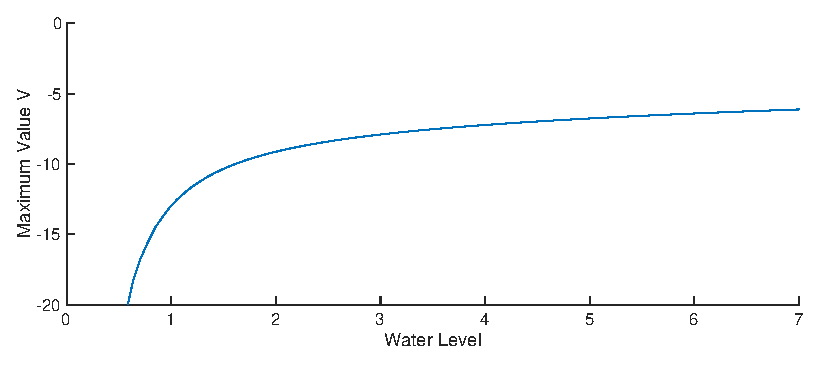
\includegraphics[width=1\textwidth]{figures/value_function.eps}
		\caption{Value Function}
		\label{fig:value-function}
	\end{figure}
	\begin{figure}[ht]
		\includegraphics[width=1\textwidth]{figures/OptimalIrrigationPolicy.eps}
		\caption{Optimal Irrigation Policy}
		\label{fig:optimal-irrigation-policy}
	\end{figure}
	\subsection{Steady State}
	\begin{figure}[ht]
		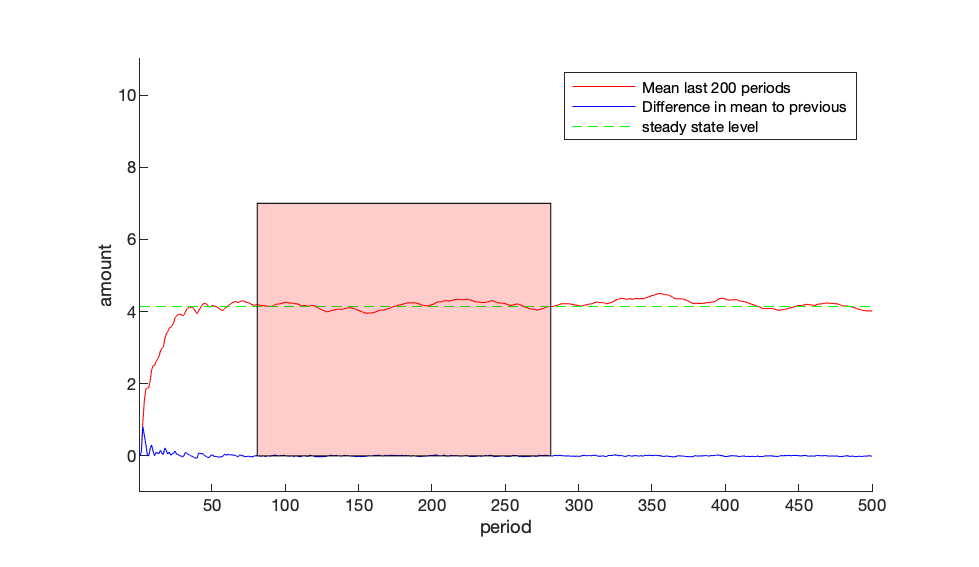
\includegraphics[width=1\textwidth]{figures/steadyState.eps}
		\caption{Exemplary Calculation of the Steady State}
		\label{fig:steadyState}
	\end{figure}
	\subsection{Steady State Probability}
	\begin{figure}[ht]
		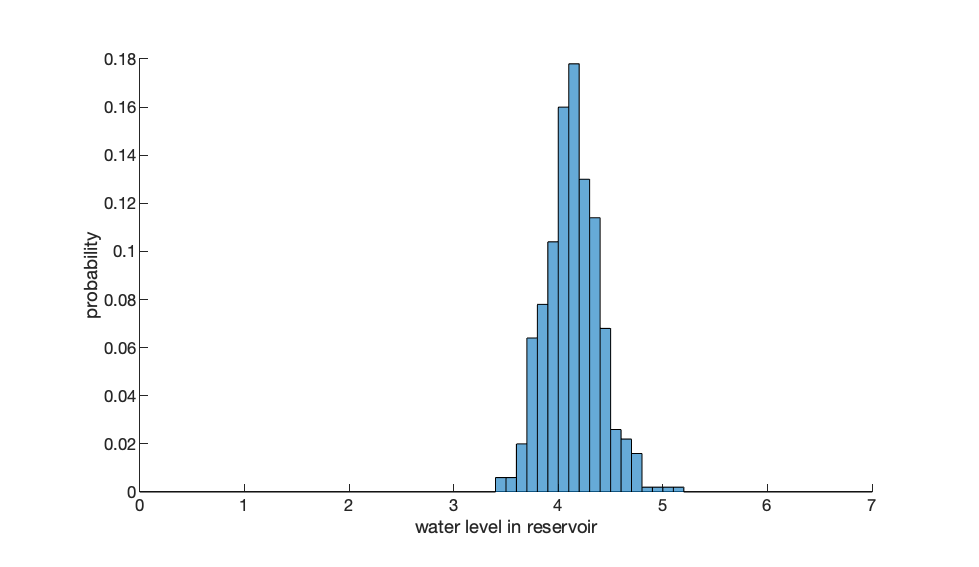
\includegraphics[width=1\textwidth]{figures/steadyStateMonteCarlo.eps}
		\caption{Steady State Probability}
		\label{fig:steadyStateMonteCarlo}
	\end{figure}
	\subsection{Effect of Changed Discount Factors to Optimal Irrigation Policy}
	\subsection{Changed Volatility of Rainfalls}

	\printbibliography

	\newpage
	
	
	%----------------------------------------------------------------------------------------
	%	STATUTORY DECLARATION IN LIEU OF AN OATH
	%----------------------------------------------------------------------------------------
	
	\begingroup
	\begin{center}
		\large
		\textbf{Eidesstattliche Versicherung}
	\end{center}
	
	\vspace{0.3cm}
	
	\begin{tabular}{@{}p{8cm}p{5.8cm}}
		\underline{\hspace{6cm}} & \underline{\hspace{5.8cm}} \\
		\vspace{0.02cm}Name, Vorname & \vspace{0.02cm}Matrikelnummer \\
	\end{tabular}
	\vspace{0.3cm}
	
	Ich versichere hiermit an Eides Statt, dass ich die vorliegende Arbeit mit dem Titel

	\begin{center}
		{\makeatletter{\emph{{\@title}}}\makeatother}
	\end{center}
	
	selbständig und ohne unzulässige fremde Hilfe erbracht habe. Ich habe keine anderen als die angegebenen Quellen und Hilfsmittel benutzt. Für den Fall, dass die Arbeit zusätzlich auf einem Datenträger eingereicht wird, erkläre ich, dass die schriftliche und die elektronische Form vollständig übereinstimmen. Die Arbeit hat in gleicher oder ähnlicher Form noch keiner Prüfungsbehörde vorgelegen.
	
	\vspace{0.6cm}
	
	\begin{tabular}{@{}p{8cm}p{5.8cm}}
		\underline{\smash{Aachen, den \today}} & \underline{\hspace{5.8cm}}\\
		Ort, Datum & Unterschrift \\
	\end{tabular}
	
	\vspace{0.6cm}

	\begin{small}
		\textbf{Belehrung:}\\
		Wer vorsätzlich gegen eine die Täuschung über Prüfungsleistungen betreffende Regelung einer Hochschulprüfungsordnung verstößt, handelt ordnungswidrig. Die Ordnungswidrigkeit kann mit einer Geldbuße bis zu 50 000 Euro geahndet werden. Zuständige Verwaltungsbehörde für die Verfolgung und Ahndung von Ordnungswidrigkeiten ist die Kanzlerin oder der Kanzler der RWTH Aachen. Im Falle eines mehrfachen oder sonstigen schwerwiegenden Täuschungsversuches kann der Prüfling zudem exmatrikuliert werden (§ 63 Abs. 5 HG NRW).
		
		\textbf{§ 156 StGB: Falsche Versicherung an Eides Statt}\\
		Wer vor einer zur Abnahme einer Versicherung an Eides Statt zuständigen Behörde eine solche Versicherung falsch abgibt oder unter Berufung auf eine solche Versicherung falsch aussagt, wird mit Freiheitsstrafe bis zu drei Jahren oder mit Geldstrafe bestraft.
		
		\textbf{§ 161 StGB: Fahrlässiger Falscheid; fahrlässige falsche Versicherung an Eides Statt}\\
		(1) Wenn eine der in den §§ 154 bis 156 bezeichneten Handlungen aus Fahrlässigkeit begangen worden ist, so tritt Freiheitsstrafe bis zu einem Jahr oder Geldstrafe ein.\\
		(2) Straflosigkeit tritt ein, wenn der Täter die falsche Angabe rechtzeitig berichtigt. Die Vorschriften des § 158 Abs. 2 und 3 gelten entsprechend
	\end{small}

	\vspace{0.6cm}
	
	Die vorstehende Belehrung habe ich zur Kenntnis genommen:
	
	\vspace{0.6cm}
	
	\begin{tabular}{@{}p{8cm}p{5.8cm}}
		\underline{\smash{Aachen, den \today}} & \underline{\hspace{5.8cm}}\\
		Ort, Datum & Unterschrift \\
	\end{tabular}
	
	\endgroup
	\clearpage
	
\end{document}
